%%%%%%%%%%%%%%%%%%%%%%%%%%%%%%%%%%%%%%%%%%%%%%%%%%%%%%%%%%%%
\documentclass[xcolor=x11names,compress]{beamer}

\definecolor{CoolBlack}{rgb}{0.0, 0.18, 0.39}
\definecolor{byellow}{rgb}{0.55037, 0.38821, 0.06142}
%% General document %%%%%%%%%%%%%%%%%%%%%%%%%%%%%%%%%%
\usepackage{graphicx}
\usepackage{tikz}
\usepackage{Tabbing}
\usetikzlibrary{decorations.fractals}
%%%%%%%%%%%%%%%%%%%%%%%%%%%%%%%%%%%%%%%%%%%%%%%%%%%%%%

%% Beamer Layout %%%%%%%%%%%%%%%%%%%%%%%%%%%%%%%%%%
\useoutertheme[subsection=false,shadow]{miniframes}
\useinnertheme{default}
\usefonttheme{serif}
\usepackage{palatino}
\usepackage{tabu}

% addition of color
\usepackage{xcolor}
\definecolor{dgreen}{rgb}{0.,0.6,0.}
\definecolor{RawSienna}{cmyk}{0,0.72,1,0.45}

\setbeamerfont{title like}{shape=\scshape}
\setbeamerfont{frametitle}{shape=\scshape}

\setbeamercolor*{lower separation line head}{bg=CoolBlack} 
\setbeamercolor*{normal text}{fg=black,bg=white} 
\setbeamercolor*{alerted text}{fg=red} 
\setbeamercolor*{example text}{fg=black} 
\setbeamercolor*{structure}{fg=black} 
 
\setbeamercolor*{palette tertiary}{fg=black,bg=black!10} 
\setbeamercolor*{palette quaternary}{fg=black,bg=black!10} 

\renewcommand{\(}{\begin{columns}}
\renewcommand{\)}{\end{columns}}
\newcommand{\<}[1]{\begin{column}{#1}}
\renewcommand{\>}{\end{column}}

% adding slide numbers
\addtobeamertemplate{navigation symbols}{}{%
    \usebeamerfont{footline}%
    \usebeamercolor[fg]{footline}%
    \hspace{1em}%
    \insertframenumber/\inserttotalframenumber
}

% equation stuff
\newcommand{\Macro}{\ensuremath{\Sigma}}
\newcommand{\Sn}{\ensuremath{S_N} }
\newcommand{\vOmega}{\ensuremath{\hat{\Omega}}}
\usepackage{mathrsfs}
\usepackage[mathcal]{euscript}
\usepackage{amssymb}
\usepackage{amsthm}
\usepackage{epsfig}
\usepackage{amsmath}

\newcommand{\ve}[1]{\ensuremath{\mathbf{#1}}}
\newcommand{\micro}{\ensuremath{\sigma}}
\newcommand{\detR}{\ensuremath{\Sigma}}
%%%%%%%%%%%%%%%%%%%%%%%%%%%%%%%%%%%%%%%%%%%%%%%%%%

\begin{document}

%%%%%%%%%%%%%%%%%%%%%%%%%%%%%%%%%%%%%%%%%%%%%%%%%%%%%%
%%%%%%%%%%%%%%%%%%%%%%%%%%%%%%%%%%%%%%%%%%%%%%%%%%%%%%
\begin{frame}
\title{Research Activities}
\subtitle{NE Dept.\ Retreat}
\author{
        \includegraphics[height=2cm]{bk}\\R.\ N.\ Slaybaugh, \\ Univ. of Cal.\ Berkeley}

\date{21 August 2014}
\titlepage
\end{frame}


% --------------------------------------------------------------
% --------------------------------------------------------------
\section{\scshape Student Projects}
\begin{frame}[fragile]
  \frametitle{Current: Warp and PyNE}

	\begin{columns}
  	\begin{column}{0.5\textwidth}
	\begin{itemize}
	  \item Kelly Rowland taking over \textbf{Warp} from Ryan Bergman
	  \item Monte Carlo on GPU
	  \item Kelly has won IUP Fellowship
	  \item Significant issue: statistical error for eigenvalue calculations
	  \item Woodcock-delta geometry tracking
	\end{itemize}
  	\end{column}
 	%
 	\begin{column}{0.5\textwidth}
 	 \begin{itemize}
       \item Josh Howland is working toward a transport solver research sandbox in \textbf{PyNE} 
       \item Wrapping a set of codes with different spatial solution methods
       \item Will add access to PyNE's existing infrastructure
       \item Becomes a``plug-and-play" toolkit
 	 \end{itemize}
  	\end{column}
	\end{columns}

\end{frame}

% --------------------------------------------------------------
\begin{frame}[fragile]
  \frametitle{Upcoming: dealing with anisotropy}

	\begin{columns}
  	\begin{column}{0.5\textwidth}
	\begin{itemize}
	\item Many important nuclear applications have strong anisotropies
	 \begin{itemize}
	 \item Used fuel casks
	 \item Reprocessing facilities
	 \item Reactor facilities
	 \item Active interrogation 
	 \end{itemize}
	\item These are difficult to capture with current tools:
	 \begin{itemize}
	 \item Ray effects with deterministic
	 \item Too slow with analog MC
	 \item Insufficient acceleration of MC with hybrid
	 \end{itemize}
	\end{itemize}
  	\end{column}
 	%
 	\begin{column}{0.5\textwidth}
 	 \begin{center}
 	 \begin{figure}
 	 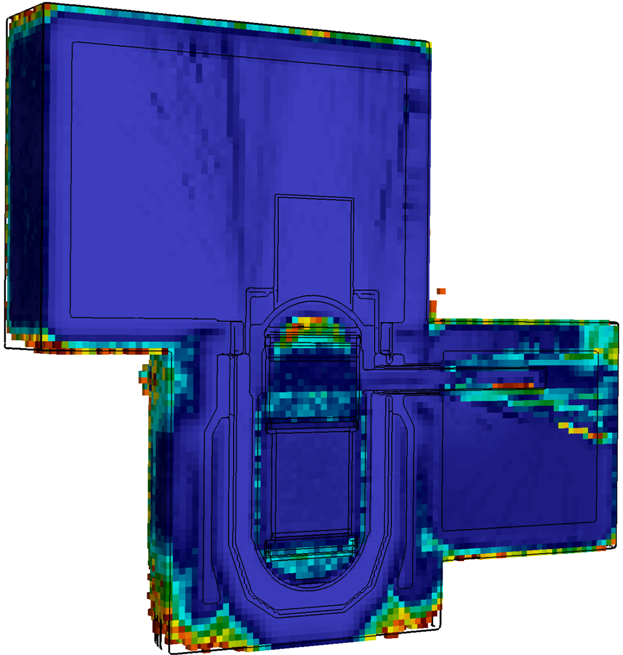
\includegraphics[height=2in,clip]{pwr}  
 	 \caption{PWR, 1 CPU-month, FW-CADIS  for mesh-tally (500K cells)}
 	 \end{figure}
 	 \end{center}

  	\end{column}
	\end{columns}

\end{frame}

% --------------------------------------------------------------
\begin{frame}[fragile]
  \frametitle{Students and Collaborators}

	\begin{itemize}
	  \item James Bevins and Madicken Munk will start working on Angle-informed VR
	  \item In collaboration with ORNL
	\end{itemize}

\end{frame}

% --------------------------------------------------------------
\begin{frame}[fragile]
  \frametitle{Current hybrid methods are insufficient}

	\begin{columns}
  	\begin{column}{0.5\textwidth}
 
  	\end{column}
 	%
 	\begin{column}{0.5\textwidth}

  	\end{column}
	\end{columns}

\end{frame}

% --------------------------------------------------------------
\begin{frame}[fragile]
  \frametitle{Better hybrid methods are needed}

	\begin{itemize}
	\item We can use angular information to improve performance
		\begin{equation}
		\phi^{\dagger}(\ve{r},E) = \frac{\int \psi(\vOmega, \ve{r},E) \psi^{\dagger}(\vOmega, \ve{r},E) d\vOmega}{\int \psi(\vOmega, \ve{r},E)  d\vOmega}
		\end{equation}

	\item The space- and energy-dependent importance map will be normalized and source biasing parameters will be generated in a manner similar to the current implementation of hybrid methods
	\item Immediately useful; widely applicable
	\end{itemize}

\end{frame}


% --------------------------------------------------------------
\begin{frame}[fragile]
  \frametitle{Lagrange Discrete Ordinate Equations}

	\begin{itemize}
	\item Re-derivation of $S_N$ with an interpolatory quadrature framework
	\item Allows evaluation at directions not on quadrature set
	\item No need to store spherical harmonic moments
	\item May be useful for more accurately capturing strong anisotropies
	\end{itemize}
	
	Use as standalone or in FW-CADIS?

\end{frame}

% --------------------------------------------------------------
% --------------------------------------------------------------
\section{\scshape Other Projects}
\begin{frame}[fragile]
  \frametitle{Other (potential) projects}

  	\begin{itemize}
  	\item Continuing development of MC on GPU
  	\item Contributing methods to PyNE; investigating a long term research relationship 
	\item 3D shielding optimization: applicable to SMRs 
	%\item Parallelization of open source deterministic code, Detran 
	\item Investigating use of hybrid methods for interrogation of SNM with neutron time-correlations 
	%\item Using SP$_N$ in multigrid preconditioner in Denovo 
	\end{itemize}
	
\end{frame}



\end{document}